 \documentclass{article}
\usepackage{tikz}
\usetikzlibrary{positioning, automata}
\usepackage{fancyhdr}
\usepackage{extramarks}
\usepackage[plain]{algorithm}
\usepackage{algpseudocode}
\usepackage[utf8]{inputenc} 
\usepackage[T1]{fontenc}    
\usepackage{hyperref}       
\usepackage{url}        
\usepackage{booktabs}
\usepackage{pdfpages}
\usepackage{amsfonts}   
\usepackage{nicefrac}       
\usepackage{microtype}      
\usepackage{amsmath}
\usepackage{graphicx}
\usepackage{float}
\usepackage{caption}
\usepackage{ragged2e}
\usepackage{amssymb}
\usepackage{mathtools}
\usepackage{xcolor}
\usepackage[spanish]{babel} % ¡Solo una vez!
\usepackage{array}
\usepackage{multirow}
\usepackage{multicol}
\usepackage{manfnt}
\usepackage{layout}
\usepackage{manfnt}
\usepackage{phaistos}
\usepackage{polynom}
\usepackage[most]{tcolorbox}
\RequirePackage{algorithm}
\RequirePackage{algpseudocode}


\setcounter{page}{0}
%
% Basic Document Settings
%

\topmargin=-0.45in
\evensidemargin=0in
\oddsidemargin=0in
\textwidth=6.5in
\textheight=9.0in
\headsep=0.25in

\linespread{1.1}
%|#*******************************************************************#|
\pagestyle{fancy}
\lhead{Taller}
\chead{\hmwkClass\ : \hmwkTitle}
\rhead{\firstxmark}
\lfoot{\lastxmark}
\cfoot{\thepage}

\renewcommand\headrulewidth{0.4pt}
\renewcommand\footrulewidth{0.4pt}

\setlength\parindent{0pt}

%
% Create Problem Sections
%

\newcommand{\enterProblemHeader}[1]{
    \nobreak\extramarks{}{Problema \arabic{#1} continúa en la siguiente página\ldots}\nobreak{}
    \nobreak\extramarks{Problema \arabic{#1} (continuación}{Problema \arabic{#1} continúa en la siguiente página\ldots}\nobreak{}
}

\newcommand{\exitProblemHeader}[1]{
    \nobreak\extramarks{Problema \arabic{#1} (continuación)}{Problema \arabic{#1} continúa en la siguiente página\ldots}\nobreak{}
    \stepcounter{#1}
    \nobreak\extramarks{Problema \arabic{#1}}{}\nobreak{}
}



\setcounter{secnumdepth}{0}
\newcounter{partCounter}
\newcounter{homeworkProblemCounter}
\setcounter{homeworkProblemCounter}{1}
\nobreak\extramarks{Problema \arabic{homeworkProblemCounter}}{}\nobreak
%margen de una pagina
\newenvironment{changemargin}[2]{%
\begin{list}{}{%
\setlength{\topsep}{0pt}%
\setlength{\leftmargin}{#1}%
\setlength{\rightmargin}{#2}%
\setlength{\listparindent}{\parindent}%
\setlength{\itemindent}{\parindent}%
\setlength{\parsep}{\parskip}%
}%
\item[]}{\end{list}}

%
% Homework Problem Environment
%
% This environment takes an optional argument. When given, it will adjust the
% problem counter. This is useful for when the problems given for your
% assignment aren't sequential. See the last 3 problems of this template for an
% example.
%
\newenvironment{homeworkProblem}[1][-1]{
    \ifnum#1>0
        \setcounter{homeworkProblemCounter}{#1}
    \fi
    \section{Problema \arabic{homeworkProblemCounter}:}
    \setcounter{partCounter}{1}
    \enterProblemHeader{homeworkProblemCounter}
}{
    \exitProblemHeader{homeworkProblemCounter}
}


%|#*******************************************************************#|

\newcommand{\hmwkTitle}{Taller 2}
\newcommand{\hmwkClass}{EDP I}
\newcommand{\hmwkUniversity}{Universidad Nacional de Colombia}
\newcommand{\hmwkAuthorName}{Edgar Santiago Ochoa Quiroga}
\newcommand{\hmwkInstructor}{\empty}

%
% Title Page
%

\title{
    \vspace{2in}
    \textmd{\textbf{\hmwkClass:\ \hmwkTitle}}\\
    \vspace{0.1in}\large{\textit{\hmwkUniversity}}\\
    \vspace{1.5in} \textrm{\hmwkInstructor}
    \vspace{1.5in}
}

\author{\hmwkAuthorName}
\date{}

\renewcommand{\part}[1]{\textbf{\large Part \Alph{partCounter}}\stepcounter{partCounter}\\}
%
%   Nuevos tipos de columna
%
\newcolumntype{C}{>{$}c<{$}}
\newcolumntype{L}{>{$}l<{$}}
\newcolumntype{R}{>{$}r<{$}}
% ---------------------------
%|  Various Helper Commands  |
% ---------------------------

% Useful for algorithms
\newcommand{\alg}[1]{\textsc{\bfseries \footnotesize #1}}

% -For derivatives-
\newcommand{\deriv}[2]{\frac{\mathrm{d #1 }}{\mathrm{d} #2} }

%For derivatives of degree >1
\newcommand{\mderiv}[3]{\frac{\mathrm{d^{#3} #1 }}{\mathrm{d} #2} }

% -For partial derivatives-
\newcommand{\pderiv}[2]{\frac{\partial}{\partial #1} (#2)}

% -Integral dx-
\newcommand{\dx}{\hspace{3pt}\mathrm{d}}

% Alias for the Solution section header
\newcommand{\solution}{\textbf{\\\\\large Solución:\\ \hspace*{5pt}}}

% Probability commands: Expectation, Variance, Covariance, Bias
\newcommand{\E}{\mathrm{E}}
\newcommand{\Var}{\mathrm{Var}}
\newcommand{\Cov}{\mathrm{Cov}}
\newcommand{\Bias}{\mathrm{Bias}}


%TcolorBox

% Definir colores y la tcolorbox de la solución
\definecolor{myDColor}{HTML}{101010} 

\definecolor{myLColor}{RGB}{153,204,255} 

\definecolor{LinkColor}{HTML}{9669d9} 


\newtcolorbox{solucion}[1][]{%
    enhanced,
    skin first=enhanced,
    skin middle=enhanced,
    skin last=enhanced,
    before upper={\parindent15pt},
    breakable,
    boxrule = 0pt,
    frame hidden,
    borderline west = {4pt}{0pt}{myDColor},
    colback = myLColor!5,
    coltitle = myLColor!5,
    sharp corners,
    rounded corners = southeast,
    arc is angular,
    arc = 3mm,
    attach boxed title to top left,
    boxed title style = {%
        enhanced,
        colback = myDColor,
        colframe = myDColor,
        top = 0pt,
        bottom = 0pt,
        sharp corners,
        rounded corners = northeast,
        arc is angular,
        arc = 2mm,
        rightrule = 0pt,
        bottomrule = 0pt,
        toprule = 0pt,
    },
    title = {\bfseries\large Solución:}, 
    overlay unbroken={%
        \node[anchor=west, color=black!70] at (title.east) {#1};
        \path[fill = tcbcolback!80!black] 
            ([yshift = 3mm]interior.south east) -- ++(-0.4,-0.1) -- ++(0.1,-0.2);
    },
    overlay first = {%
        \node[anchor=west, color=black!70] at (title.east) {#1};
        \path[fill = tcbcolback!80!black] 
            ([yshift = 3mm]interior.south east) -- ++(-0.4,-0.1) -- ++(0.1,-0.2);
    },
    overlay middle={%
        \path[fill = tcbcolback!80!black] 
            ([yshift = -3mm]interior.north east) -- ++(-0.4,0.1) -- ++(0.1,0.2);
        \path[fill = tcbcolback!80!black] 
            ([yshift = 3mm]interior.south east) -- ++(-0.4,-0.1) -- ++(0.1,-0.2);
    },
    overlay last={%
        \path[fill = tcbcolback!80!black] 
            ([yshift = -3mm]interior.north east) -- ++(-0.4,0.1) -- ++(0.1,0.2);
        \path[fill = tcbcolback!80!black] 
            ([yshift = 3mm]interior.south east) -- ++(-0.4,-0.1) -- ++(0.1,-0.2);
    },
    extras middle and last = { rounded corners = northeast }
}
\newcommand{\qed}{\hfill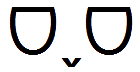
\includegraphics[height=2ex]{Demo_face-removebg-preview .png}}
\usepackage{amsmath}
\usepackage{geometry}
\usepackage{tikz}
\usepackage{float}
\usepackage{graphics}

\tikzset{every picture/.style={line width=0.75pt}} %set default line width to 0.75pt        

\begin{document}
\maketitle
\thispagestyle{empty}
\newpage 

\begin{homeworkProblem}
    Las clases de conjugación de $S_n$ corresponden a particiones de $n,$ dadas por la longitud de los ciclos. Determine el tamaño de la clase de conjugación de en $S_n$ que corresponde a una partición dada $n=\sum jm_j.$ ($m_1$ elementos fijos, $m_2$ 2-ciclos, $m_3$ 3-ciclos$\dots$ )
    \begin{solucion}
     Como el tamaño de la clase de conjugación corresponde a la partición particular de $n$ que define el tipo de ciclo. entonces basta con ver de cuantas maneras se puede escribir ese ciclo en particular para determinar el tamaño de la clase de conjugación. Primero es claro que en los ciclos independientemente de su distribución podemos asegurar que hay $n!$ maneras de colocar los elementos de $\{1,2,3\dots,n\}$. Ahora hay que ver cuantas maneras repetidas tenemos que descontar. Fijemos un tipo de ciclo especifico en el cual hay una cantidad $m_1$ de 1-ciclos, $m_2$ de 2-ciclos y así sucesivamente. Observe que en un $j$-ciclo especifico se puede escribir de $j$ maneras diferentes desplazando los elementos una posición sin alterar su orden para cada $j$-ciclo, y como hay una cantidad $m_j$ de esos ciclos, se obtiene que de momento hay $j^{m_j}$ casos repetidos, pero falta tener en cuenta una cosa, note que los $j$-ciclos como hay una cantidad $m_j$ de ellos puedo permutarlos sin alterar la permutación, entonces habrían $m_j!$ maneras de permutarlos y junto con lo anterior para un tipo de ciclo especifico tendríamos que hay $m_j!j^{m_j}$ maneras distintas de escribirlo sin alterar la permutación. Luego como esto es para cada $j$-ciclo pues basta con multiplicar todos estos y dividir esta cantidad a $n!$. Así obtenemos que el tamaño de una clase de conjugación correspondiente a una partición es:
     $$\frac{n!}{(m_1!1^{m_1})(m_2!2^{m_2})\dots(m_n!n^{m_n})}$$
     Note que en los casos que hay 0 ciclos de algún $j-$ciclo especifico ese termino en particular se hace 1 y no afecta el resultado.

     \qed
     \end{solucion}
\end{homeworkProblem}
\newpage
\begin{homeworkProblem}
    Pruebe que $A_n$ es generado por 3-ciclos. Usando este hecho pruebe que $A_n$ es simple.
    \begin{solucion}
    Primero probemos que $A_n$ es generado por 3-ciclos para $n\geq 3$.\\
    Sea $X$ el conjunto de todos los 3-ciclos y sea $\sigma=(a,b,c)$ con $a,b,c\in\{1,2,3,\dots,n \}$, es claro que $(a,b,c)=(a,c)(a,b)$ por tanto $\sigma\in A_n$ y como este era arbitrario $\langle X\rangle\subseteq A_n$. Ahora sea $\sigma\in A_n$, por definición $\sigma$ se puede escribir como un numero par de trasposiciones, es decir $\sigma=\tau_1\tau_2\dots\tau_k$ con $k$ par y donde cada $\tau_i=(a_1,a_2)$ con $a_1,a_2\in\{1,2,3,\dots,n \}$ y $a_1\neq a_2$, note que podemos agrupar trasposiciones dos a dos. Veamos que el producto de 2 trasposiciones puede ser visto como el producto de 3-ciclos. Sean $(a,b)$ y $(c,d)$ dos trasposiciones tenemos dos casos posibles:
    \begin{itemize}
        \item Caso 1: $\{a,b\}\cap\{c,d\}=\varnothing$, es decir son ciclos disyuntos y por tanto tenemos que:
        \begin{align*}
            (a,b)(c,d)&=(a,b)id(c,d)\\
            &=(a,b)[(b,c)(b,c)](c,d)\\
            &=(a,b)(b,c)(c,d,b)\\
            &=(a,b,c)(c,d,b)
        \end{align*}
        \item Caso 2: $\{a,b\}\cap\{c,d\}\neq\varnothing$, es decir coinciden en algunos elementos, o en todos, veamos que posibilidades hay.\\
        La primera es que $\{a,b\}=\{c,d\}$, es decir $(a,b)=(c,d)$ y por tanto:
        $$(a,b)(c,d)=(a,b)(a,b)=id=(a,b,r)(a,b,r)(a,b,r)$$
        donde $r$ es un elemento distinto a $a,b$, note que esto lo podemos asegurar ya que $n\geq 3$.
        Ahora como segundo caso consideremos que $a=c$ pero $b\neq d$, por tanto tenemos que:
        $$(a,b)(c,d)=(a,b)(a,d)=(a,d,b)$$
        Por ultimo tendríamos el caso $a=d$ y $b\neq c$ que es análogo al anterior:
        $$(a,b)(c,d)=(a,b)(c,a)=(a,c,b)$$
        \end{itemize}
        De esta forma concluimos que cualquier producto dos a dos de trasposiciones es un producto de 3-ciclos, luego $\sigma$ es un producto de tres ciclos, por lo tanto $\sigma\in\langle X\rangle$ y $A_n\subseteq\langle X\rangle$. Por la doble contenencia concluimos que $A_n$ es generado por los 3-ciclos.
        Ahora debemos mostrar que si $N\trianglelefteq A_n$, para $n\geq 5$ y $N$ contiene un 3-ciclo, entonces $N=A_n$. Para esto primero demostremos que todos los 3-ciclos son conjugados en $S_n$, por medio de la identidad $f(a,b,c)f^{-1}=(f(a),f(b),f(c))$. Sea $(a,b,c)$ un 3-ciclo arbitrario y sea $f\in S_n$ una permutación arbitraria. Ahora como $f$ puede ser escrita como producto de trasposiciones basta con ver que pasa en el caso de que $f$ sea un ciclo de la forma $(\alpha,\beta)$ y nuevamente consideraremos dos casos:
        \begin{itemize}
            \item Caso 1: $\{\alpha,\beta\}\cap\{a,b,c\}=\varnothing$, quiere decir que son disyuntos y por tanto conmutan los ciclos:
            $$(\alpha,\beta)(a,b,c)(\alpha,\beta)=(a,b,c)(\alpha,\beta)(\alpha,\beta)=(a,b,c)$$
            Note que podemos ver $(a,b,c)=(f(a),f(b),f(c))$ ya que $f$ no mueve estos elementos.
            \item Caso 2: $\{\alpha,\beta\}\cap\{a,b,c\}\neq\varnothing$, y tenemos dos casos, el primero suponga que $\alpha,\beta\in\{a,b,c\}$ y que $\alpha=a$ y $\beta=b$, tenemos que:
            $$(\alpha,\beta)(a,b,c)(\alpha,\beta)=(a,b)(a,b,c)(a,b)=(b,a,c)=(f(a),f(b),f(c))$$ y en caso de que $\alpha=a$ y $\beta=c$:
            $$(\alpha,\beta)(a,b,c)(\alpha,\beta)=(a,c)(a,b,c)(a,c)=(c,b,a)=(f(a),f(b),f(c))$$
        \end{itemize}
        Esto agota las posibilidades y por tanto muestra que los 3-ciclos son conjugados en $S_n$. Ahora para probar esto en $A_n$ basta con ver que la permutación $f$ siempre la podemos tomar par. Si $f$ es par no hay nada que probar. Consideremos $f$ impar, como $n\geq 5$ existen $i,j$ diferentes a $a,b,c$ y por tanto sus ciclos conmutaran, luego planteemos que la permutación par que conjuga es $\pi=f(i,j)$, de esta manera:
            $$(f(i,j))(a,b,c)(f(i,j))^{-1}=f(i,j)(a,b,c)(i,j)f^{-1}=f(a,b,c)(i,j)(i,j)f^{-1}=f(a,b,c)f^{-1}$$
            y que por lo anterior podemos concluir que todos los 3-ciclos son conjugados en $A_n$ para $n\geq 5$.
            Ahora volvamos a lo que realmente nos interesaba probar. Como $N$ contiene un 3-ciclo y es normal, los conjugados de ese 3-ciclo pertenecen a $N$, es decir $N$ contiene todos los 3-ciclos y como $A_n$ es generado por estos no queda de otra que $N=A_n$.\\

            Con todo esto ya podemos probar lo que nos interesa, $A_n$ es simple para todo $n\geq 5$.
            Sea $N\trianglelefteq A_n$ y supongamos que $N\neq\{id\}$, es decir hay un $\tau\in N$ distinto a la identidad. Vamos a mostrar que la existencia de tal elemento implica que en $N$ hay un 3-ciclo y por tanto que es todo $A_n$, esto sera por casos:
            \begin{itemize}
                \item Caso 1: En la descomposición en ciclos disyuntos de $\tau$ hay al menos un $r$-ciclo con $r\geq 4$, es decir $\tau=(a_1,a_2,a_3,a_4,\dots,a_r)\cdots$ donde los puntos suspensivos indican la existencia de otros ciclos. Consideremos $\sigma=(a_1,a_2,a_3)\in A_n$ como $N$ es un subgrupo normal $\sigma\tau\sigma^{-1}\tau^{-1}\in N$ pero note que esto es:
                \begin{align*}
                   \sigma\tau\sigma^{-1}\tau^{-1}&=(a_1,a_2,a_3)(a_1,a_2,a_3,a_4,\dots,a_r)\cdots(a_3,a_2,a_1)\cdots(a_r,\dots,a_4,a_3,a_2,a_1)\\
                   &=(a_1,a_2,a_4)\in N
                \end{align*}
                De esta manera $N$ contiene un 3-ciclo y por lo anterior $N=A_n$
                \item Caso 2: $\tau$ contiene al menos un 3-ciclo y los demás son de longitud menor o igual a 3. Es decir $\tau=(a_1,a_2,a_3)(a_4,a_5,\cdots)\cdots$, y consideremos $\sigma=(a_1,a_2,a_4)\in A_n$ igual que en el anterior $\sigma\tau\sigma^{-1}\tau^{-1}\in N$ y:
                \begin{align*}
                    \sigma\tau\sigma^{-1}\tau^{-1}&=(a_1,a_2,a_4)(a_1,a_2,a_3)(a_4,a_5,\cdots)\cdots(a_4,a_2,a_1)\cdots(\cdots,a_5,a_4)(a_3,a_2,a_1)\\
                    &=(a_1,a_2,a_5,a_3,a_4)\in N
                \end{align*}
                y por el Caso 1, tenemos que hay un 3-ciclo en $N$ y nuevamente concluimos que $N=A_n$
                \item Caso 3: $\tau$ es exactamente un 3-ciclo y por tanto no hay nada que probar ya que $N$ ya tendría un 3-ciclo y por tanto $N=A_n$
                \item Caso 4: En $\tau$ todos los ciclos son de longitud menor o igual a $2$, es decir $\tau=(a_1,a_2)(a_3,a_4)\dotsc$. Considere $\sigma=(a_1,a_2,a_3)\in A_n$, nuevamente $\sigma\tau\sigma^{-1}\tau^{-1}\in N$ y:
                \begin{align*}
                    \sigma\tau\sigma^{-1}\tau^{-1}&=(a_1,a_2,a_3)(a_1,a_2)(a_3,a_4)\dotsc(a_3,a_2,a_1)(a_1,a_2)(a_3,a_4)\dotsc\\
                    &=(a_1,a_3)(a_2,a_4)\in N
                \end{align*}
                Ahora como $n\geq 5$ tenemos que:
                $$(a_1,a_2,a_5,a_3,a_4)=(a_1,a_4)(a_1,a_3)(a_1,a_5)(a_1,a_2)\in A_n$$
                y como $N$ es normal:
                $$(a_1,a_2,a_5,a_3,a_4)(a_1,a_3)(a_2,a_4)(a_4,a_3,a_5,a_2,a_1)=(a_1,a_5)(a_2,a_4)\in N$$
                y por ultimo al hacer el producto de esos dos elementos de $N$ obtenemos:
                $$(a_1,a_3)(a_2,a_4)(a_1,a_5)(a_2,a_4)=(a_1,a_5,a_3)\in N$$
                Por lo que hay un 3-ciclo en $N$ y así concluimos que $N=A_n$
            \end{itemize}
            Como hemos agotado todas las posibilidades concluimos que $A_n$ para $n\geq 5$ es simple. Cabe aclarar que los casos con $n=1,2,3$ también determinan a $A_n$ simple de manera trivial y que el caso $n=4$ vimos en clase como no era simple.
            
            \qed
    \end{solucion}
\end{homeworkProblem}
\newpage
\begin{homeworkProblem}
    Clasifique los grupos de orden 12.
    \begin{solucion}
    Primero por el Teorema de Clasificación (o estructura) de lo Grupos abelianos finitos tenemos que si $|G|=12$ y $G$ es abeliano entonces:
    \begin{align*}
G\cong\mathbb{Z}_4\times\mathbb{Z}_3\cong\mathbb{Z}_{12}&&\text{ó}&&G\cong\mathbb{Z}_2\times\mathbb{Z}_2\times\mathbb{Z}_3\cong\mathbb{Z}_2\times\mathbb{Z}_6
    \end{align*}
    Ahora veamos que ocurre cuando $G$ es no abeliano.\\

    Tomemos $H$ un 3-subgrupo de Sylow de $G$, es decir $H=\langle c\rangle$ para algún $c\in G$ y $|H|=3$, Ahora definamos el siguiente homomorfismo (Generalización del teorema de Caley presentada en los cuadernos de álgebra del profesor Lezama):
    $$\varphi:G\longrightarrow Sym(G/H)$$
    De tal manera que $\varphi(x)=\varphi_x$ donde:
    $$\varphi_x:G/H\longrightarrow G/H$$
    tal que $\varphi_x(gH)=xgH$. Observe que $|G/H|=4$ y por tanto $Sym(G/H)\cong S_4$. Ahora note que el ker$(\varphi)\subseteq H$ y por tanto ker$(\varphi)=\{e\}$ o ker$(\varphi)=H$. en el primer caso tendríamos que $G$ es isomorfo a un subgrupo de $S_4$ de orden 12, llamémoslo $K$, Note que $[S_4:K]=2$ por tanto $K$ es normal, Ya conocemos que $A_4$ tiene orden $12$ toca ver que nuestro $K$ es igual a $A_4$. en este caso tenemos dos posibilidades $K$ tiene un 3-ciclo o no lo tiene. Si lo tiene por el punto anterior concluimos que $K=A_4$, Ahora veamos que no es posible lo segundo. Sea $\sigma\notin K$ un 3-ciclo, Note que las clases $K,\sigma K, \sigma^{-1}K$ son distintas eso nos daría que $[S_4:K]\geq 3$ una contradicción. Así concluimos que en este caso tenemos que $G\cong A_4$. Ahora supongamos que ker$(\varphi)=H$, luego $H$ es normal en $G$ y por tanto es el único 3 subgrupo de Sylow, entonces solo hay dos elementos de orden 3, $c,c^2$. Ahora como los elementos conjugados tienen el mismo orden y $H$ es normal entonces $|O(c)|\in\{1,2\}$, donde la orbita esta definida por la conjugación de elementos, de esto tenemos por la ecuación de clases que $|C_G(c)|\in\{6,12\}$, pero en cualquiera de los dos casos existe un elemento $d$ de orden 2, y como $cd=dc$, digamos que $a:=cd$, note que $|a|=6$, luego $[G:\langle a\rangle]=2$ y por tanto $\langle a\rangle\trianglelefteq G$. Consideremos $b\in G$ tal que $b\notin\langle a\rangle$, note que $b^2\in\langle a\rangle$, además como este es normal $bab^{-1}\in\langle a\rangle$. Observemos los posibles casos:
    \begin{itemize}
        \item $bab^{-1}=e$ por tanto $a=e$, lo cual es falso
        \item $bab^{-1}=a$ por tanto $ba=ab$, pero $\langle a,b\rangle$ posee 12 elementos y por tanto $G$ seria abeliano, lo cual es falso.
        \item $bab^{-1}=a^2$, así $(bab^{-1})^3=a^6=1$, luego $ba^3b^{-1}=1$ y por tanto $a^3=1$, lo cual es falso.
        \item $bab^{-1}=a^3$, así $(bab^{-1})^2=a^6=1$, luego $ba^2b^{-1}=1$ y por tanto $a^2=1$, lo cual es falso.
        \item $bab^{-1}=a^4$ así $(bab^{-1})^3=a^12=1$, luego $ba^3b^{-1}=1$ y por tanto $a^3=1$, lo cual es falso.
        \item $bab^{-1}=a^5=a^{-1}$, como esta es la única posibilidad restante se vuelve una condición necesaria.
    \end{itemize}
    Ahora veamos los casos de valores para $b^2$:
    \begin{itemize}
        \item $b^2=1$ es una posibilidad
        \item $b^2=a$ implica que $b^12=a^6=1$ por tanto $|b|\,|12$
        \begin{itemize}
            \item $|b|=1$, entonces $b=e$, es falso.
            \item $|b|=2$ entonces $e=b^2=a$, es falso.
            \item $|b|=3$ entonces $e=b^2b=ab$ por lo que $b\in\langle a\rangle$ lo cual es falso.
            \item $|b|=4$ entonces $e=b^4=a^2$, es falso.
            \item $|b|=6$ entonces $e=b^6=a^3$, es falso.
            \item $|b|=12$ entonces $<b>=G$, $G$ es no abeliano por tanto es falso.
        \end{itemize}
    \item $b^2=a^2$, note que $a^{-2}=(bab^{-1})^2=ba^2b^{-1}=bb^2b^{-1}=b^2=a^2$ por tanto $a^4=1$, es falso.
    \item $b^2=a^3$ es una posibilidad.
    \item $b^2=a^4$, note que $a^{-4}=(bab^{-1})^4=ba^4b^{-1}=bb^2b^{-1}=b^2=a^4$ por tanto $a^8=1$ y $6|8$, es falso.
    \item $b^2=a^5$ note que $a^{-5}=(bab^{-1})^5=ba^5b^{-1}=bb^2b^{-1}=b^2=a^5$ por tanto $a^{10}=1$ y $6|10$, es falso.
    \end{itemize}
    Ahora antes de establecer las condiciones finales veamos que el conjunto:
    $$C:=\{a^kb^m|0\leq k\leq 5,0\leq m\leq 1\}$$
    tiene 12 elementos. Tome $k_1,k_2$ y $m_1,m_2$ tales que $a^{k_1}b^{m_1}=a^{k_2}b^{m_2}$, de aquí tenemos que $a^{k_1-k_2}=b^{m_2-m_1}$, supongamos que $m_2>m_1$ luego $b=a^{k_1-k_2}\in\langle a\rangle$ lo cual es falso. De aquí concluimos que $m_1=m_2$ y $k_1=k_2$. Así $C$ tiene 12 elementos. por tanto $\langle a,b\rangle\cong G$. Para finalizar según todo lo anterior determinamos que si $G$ es no abeliano tenemos alguno de los siguientes casos:
    \begin{itemize}
        \item $G\cong A_4$
        \item $G\cong\langle a,b | a^6=1, b^2=1, bab^{-1}=a^{-1}\rangle$
        \item $G\cong\langle a,b | a^6=1, b^2=a^3, bab^{-1}=a^{-1}\rangle$
    \end{itemize}
    Así concluimos que para los grupos de orden 12 hay 2 abelianos y 3 no abelianos.

    \qed
    \end{solucion}
\end{homeworkProblem}

\newpage
\begin{homeworkProblem}
    Sea $PSL_2(\mathbb{Z})=SL_2(\mathbb{Z})/\{\pm I\}$. Muestre que $PSL_2(\mathbb{Z})\simeq\langle SR,S^2,R^3\rangle$ donde
    $$S=\begin{pmatrix}
          0 & -1\\
          1 & 0
        \end{pmatrix} \text{ y }
        R=\begin{pmatrix}
            0 & -1\\
            1 & 1
        \end{pmatrix}$$
        \begin{solucion}
        Esta proposición es falsa, veamos por que.
        Primero observe que:
        $$S^2=\begin{pmatrix}
          0 & -1\\
          1 & 0
        \end{pmatrix}\begin{pmatrix}
          0 & -1\\
          1 & 0
        \end{pmatrix}=\begin{pmatrix}
          -1 & 0\\
          0 & -1
        \end{pmatrix}$$
        y además:
        $$R^3=\begin{pmatrix}
            0 & -1\\
            1 & 1
        \end{pmatrix}\begin{pmatrix}
            0 & -1\\
            1 & 1
        \end{pmatrix}\begin{pmatrix}
            0 & -1\\
            1 & 1
        \end{pmatrix}=\begin{pmatrix}
            -1 & -1\\
            1 & 0
        \end{pmatrix}\begin{pmatrix}
            0 & -1\\
            1 & 1
        \end{pmatrix}=\begin{pmatrix}
            -1 & 0\\
            0 & -1
        \end{pmatrix}$$
        Es decir que $S^2=R^3=-I$, Además:
        $$SR=\begin{pmatrix}
          0 & -1\\
          1 & 0
        \end{pmatrix}\begin{pmatrix}
            0 & -1\\
            1 & 1
        \end{pmatrix}=\begin{pmatrix}
            -1 & -1\\
            0& -1
        \end{pmatrix}=-1\begin{pmatrix}
            1 & 1\\
            0& 1
        \end{pmatrix}$$
        Llamemos $SR=T$ ahora podemos probar por inducción que:
        $$(T)^n=(-1)^n\begin{pmatrix}
            1 & n\\
            0& 1
        \end{pmatrix}$$
        Observe que para $n=1$ se tiene el resultado, Ahora supóngalo para $n$ y veamos que ocurre con $n+1$
        $$(T)^{n+1}=T^nT=(-1)^n\begin{pmatrix}
            1 & n\\
            0& 1
        \end{pmatrix}(-1)\begin{pmatrix}
            1 & 1\\
            0& 1
        \end{pmatrix}=(-1)^{n+1}\begin{pmatrix}
            1 & n+1\\
            0& 1
        \end{pmatrix}$$
        Entonces tenemos que:
        $$\langle SR,S^2,R^3\rangle=\left\langle(-1)^{n+1}\begin{pmatrix}
            1 & n+1\\
            0& 1
        \end{pmatrix},-I\right\rangle$$
        Ahora note que $S,R\in PSL_2(\mathbb{Z})$ por definición, pero ni $S$ ni $R$ pueden ser generadas por $\langle SR,-I\rangle$ por lo que no pueden ser isomorfas.
        
        \qed
        \end{solucion}
        
\end{homeworkProblem}

%%%%%%%%%%%%%%%%%%%%%%%%%%%%%%%%%%%%%%%%%%%%%%%%%%%%%%%
\end{document}